\RequirePackage{plautopatch}
\documentclass[uplatex,a4paper,11pt]{jsarticle}

% 数式
\usepackage{amsmath,amsfonts}
\usepackage[dvipdfmx]{graphicx}
\usepackage{bm}
\usepackage{ulem}
% 画像
\usepackage[dvipdfmx]{graphicx}

\begin{document}

\title{JPHACKSにおける音声特徴量抽出技術の開発}
\author{Application Bug Creater 2021}
\date{\today}
\maketitle

\section{はじめに}
時は昨年に遡る.筆者は,素晴らしい(クレイジーな)メンバーと共にJPHACKSで開発できて満足していた.
そして,来年は研究が忙しくなり,ハッカソンに全力で打ち込むことはおろか,参加すら怪しくなると思っていた.

ところが実態はどうであろうか.今年の制作物は,似ている音声ファイルの検索となっ(てしまっ)た.
もちろんライブラリなどなく,似たサービス(曲を除く)もなく,論文でようやく見るぐらいだ.

今年も楽しい\sout{研究}ハッカソンの始まりだ.

\section{導入}
\subsection{音の理論}
そもそも音とは何であろうか.音とは,空気の疎密波である.よく音は波とよばれるが,空気の密度の疎な部分と密な部分が移動していくことで音というものが伝わっていく.
それでは,人はどのようにその波を音として認識するのか.それは,耳の奥にある鼓膜が,空気の疎密波によって振動し,蝸牛でその振動を聴覚神経に電気信号に変換することで,人は音を認識する.
蝸牛は,音の周波数によってそれぞれ共振する場所がある.その共振を聴覚神経が感じることで音というものを聴くことができる.

つまり,音は周波数によって聴いているのである.では,音色とは何か.また,どのように分析すればよいのだろうか.

\subsection{先行研究}
筆者は信号処理の知識はあるが,現在の音の特徴量抽出についての知識は無かったため, 既存技術の調査を行った. 以下はその代表的なものである.

\subsubsection{パワースペクトル密度}
先ほど,音は周波数によって聴いていると書いた.では,音を周波数ごとに分ければ音色の本質に近づくであろうことは自然だ.
そのために,以下のような変換を用いる.
\begin{enumerate}
  \item フーリエ変換 Fourier transform (FT)
  \item 離散フーリエ変換 discrete Fourier transform (DFT)
\end{enumerate}
コンピューター上のオーディオである以上,DFTを用いることになる.DFTを用い,音を周波数ごとに分けると以下の図\ref{fig:psd}のようになる.
(DFTの結果の絶対値の二乗をパワースペクトル密度という.)なお,DFTの詳細については後述する.

\subsubsection{フォルマント}
図\ref{fig:psd}を見てもらえればわかるが,データとして多く,特徴検索に向かない.
そこで,図\ref{fig:envelope}のような包絡線を描き,ピークとなるところ(青色で囲ったところ)で左側にある順から第一フォルマント・第二フォルマント…と呼ぶ.\cite{iroha}
こうすることで,音色というものを大きく圧縮することができる.

この特徴量は音声認識においてよく用いられ,フォルマントを調整することによって男性っぽい声・女性っぽい声と変えることができる.

\subsubsection{離散全極型モデル}
フォルマントは,非常に音を圧縮した表現となり,音声認識では問題ないが,音色としては逆に特徴量を捨てすぎているという問題がある.そこで,離散全極型モデル\cite{parts}というものがある.
これは,パワースペクトル密度とフォルマントの中間的な表現であり,以下の図\ref{fig:dap}で示すように,音の周波数ごとのピーク値と音量を特徴量としたものである.
この方式であれば,充分音色を表現でき,かつ,よく圧縮できている.

\begin{figure}[h]
  \begin{tabular}{cc}
    \begin{minipage}[t]{0.33\hsize}
      \centering
      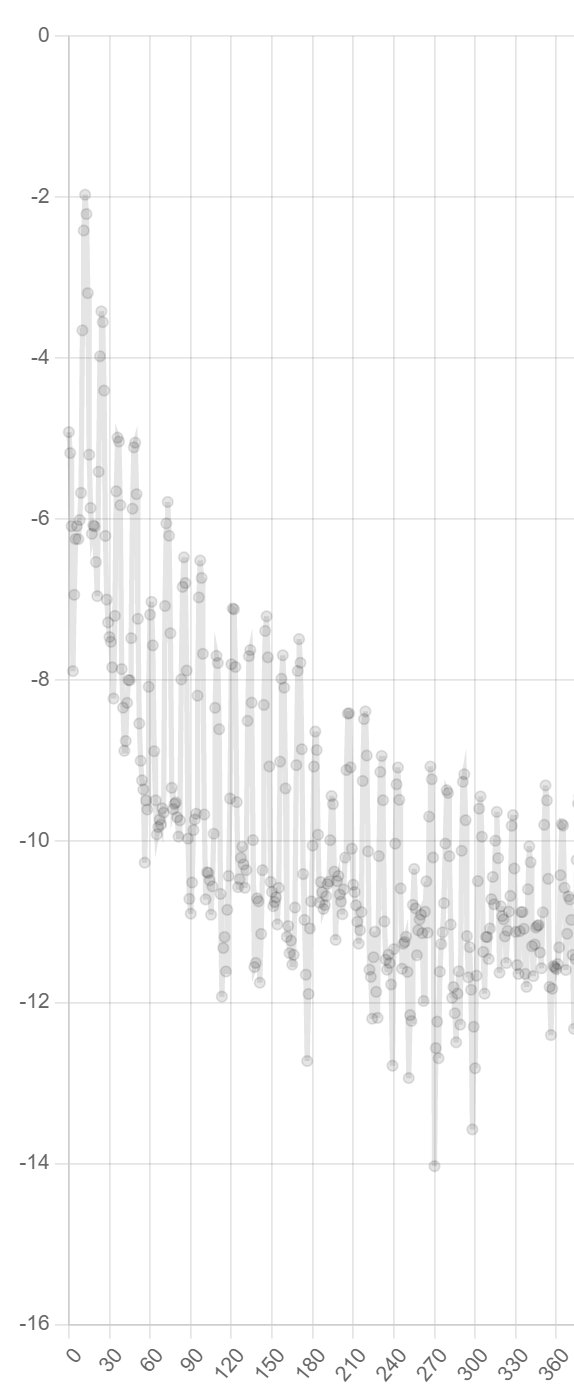
\includegraphics[width=40mm]{picture/power_spectra.png}
      \caption{パワースペクトル密度}
      \label{fig:psd}
    \end{minipage}
    \begin{minipage}[t]{0.33\hsize}
      \centering
      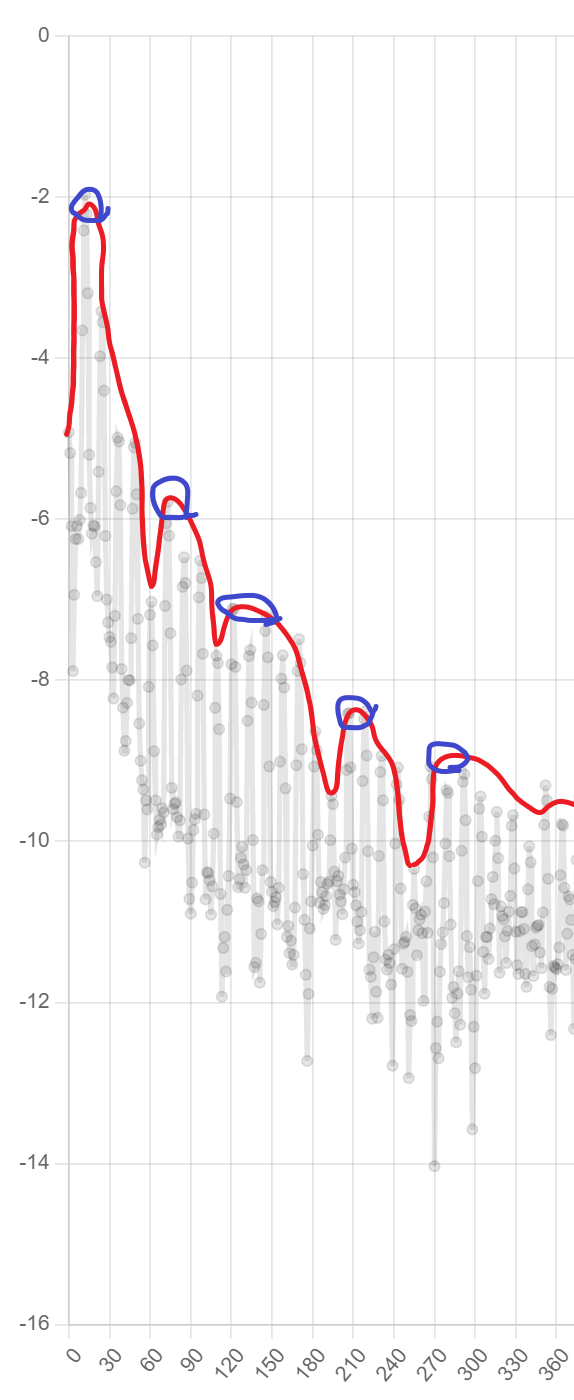
\includegraphics[width=40mm]{picture/envelope.png}
      \caption{包絡線}
      \label{fig:envelope}
    \end{minipage}
    \begin{minipage}[t]{0.33\hsize}
      \centering
      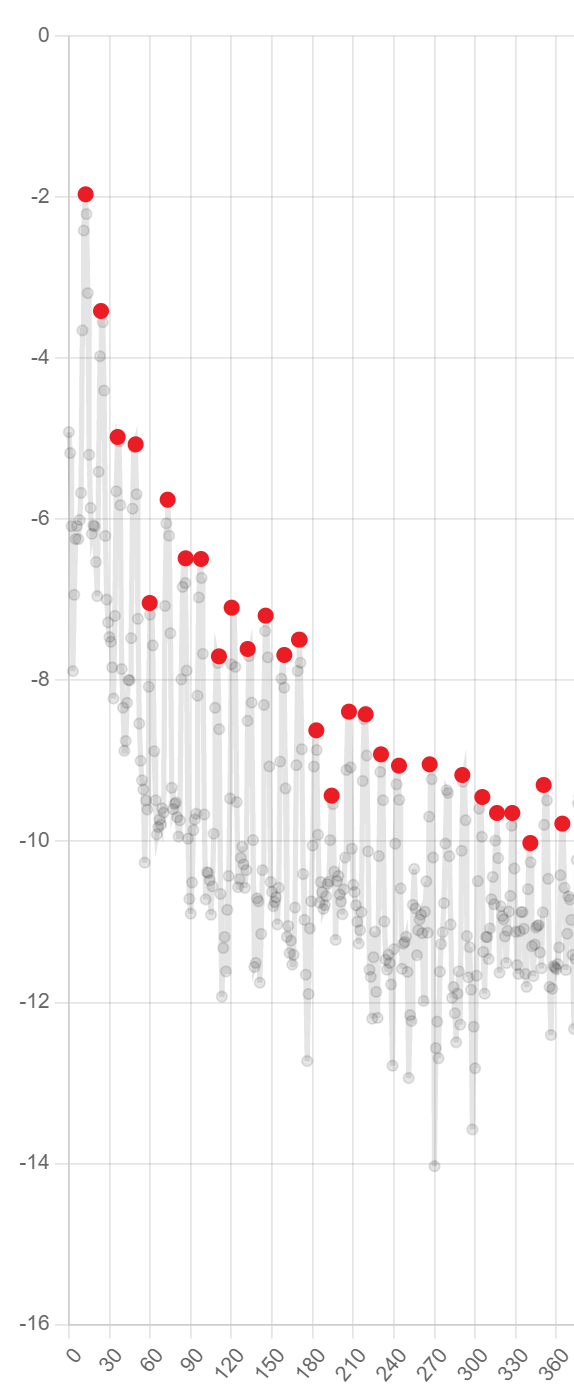
\includegraphics[width=40mm]{picture/dap.png}
      \caption{離散全極型モデル}
      \label{fig:dap}
    \end{minipage}
  \end{tabular}
\end{figure}

\subsubsection{相互相関}
ふたつの信号がどれだけ似ているかというものに,以下の式で表されるような相互相関関数がよく用いられる.
\begin{displaymath}
  (f*g)(m) = \sum_n f(n)g(m-n)
\end{displaymath}
この関数の意味としては,時間
\begin{math}
  m
\end{math}
だけシフトした際にどれだけ信号が似ているかというものである.
そのため,この関数の最大値が大きいほど似た信号と判断できる.

しかし,相互相関は音の高さが異なると相関は低いと判定してしまうため,今回の音色を探すという目的には合わない.


\section{特徴量抽出方針}
先行研究の離散全極型モデルを元に,更に発展させる方針とする.

\subsection{用いる公式}
以下では,重要な式を紹介する.

\subsubsection{DFT}
離散データを周波数領域に変換する離散フーリエ変換.
\begin{displaymath}
  F(t) = \sum^{N-1}_{x=0} f(x)exp(-j \frac{2\pi tx}{N})  
\end{displaymath}

\subsubsection{窓関数}
無限時間のDFTであれば目的のパワースペクトル密度を得られるが,現実には有限時間で区切る必要がある.
そのため,目的以外の周波数であるサイドロープが付随してしまう.そこで,窓関数を用いることで,サイドロープを減少させる.
窓関数を使うことでサイドロープを減少するが,周波数分解能が下がるが,これは提案手法によって克服される.
なお,今回用いたのはブラックマン‐ナットール窓で,サイドロープの減少幅が大きい.
\begin{displaymath}
  w(x)=0.3635819-0.4891775\cos (2\pi x) +0.1365995\cos (4\pi x)-0.0106411\cos (6\pi x)
\end{displaymath}

\subsubsection{FFT}
DFTについて紹介したが,計算量が\begin{math}
  O(n^2)
\end{math}
と大きい.しかし,高速フーリエ変換によって計算量を\begin{math}
  O(n \log n)
\end{math}
に抑えることができる.

\subsubsection{STFT}
現実には,同じ音がなり続けるということはなく,変わっていくものである.
そこで,短い期間で時間をずらしながらFFTすることによって,音の変化も観測できる.
これを短時間フーリエ変換と呼ぶ.

\section{提案手法}
我々が提案する手法は,短期間と長期間の二種類のSTFTをして,離散全極型モデルの特徴量を抽出する.
そして,短期間の物を中心にし,特徴量の補正をし,最も音色であると考えられる特徴量を選択する.
この得られた特徴量を,基本周波数・電力で正規化したものを特徴量とする.
これはベクトル表現でき,特徴量ベクトル間の距離を音色の近さの指標として提案する.

\subsection{特徴量の補正}

\subsection{隣接する短期間STFT}
短期間の窓は0.1秒ほどであるため,隣接するSTFTの要素は,ほぼ同じ音が鳴っていると考えられる.
その性質を利用し,ノイズに埋もれたピークを取り出すことが可能である.
具体的には,音量が小さい方のものに大きい方の特徴量をスケールし,ノイズと判定する閾値を下回れば,
ノイズに埋もれたピークと判断し追加することで取り出すことができる.

\subsubsection{短期間と長期間STFTの組み合わせ}
短期間STFTは短い期間を分析でき,長期間STFTは周波数分解能が高いといった特徴を持つ.
まず,短期間STFTで音色の特徴量の候補を抽出する.
そして,その短期間STFTが所属する長期間STFTの特徴量で補正することができる.
このように,ふたつを組み合わせることで双方の利点を利用できる.

\subsubsection{楽器の性質}
いわゆる物理的な楽器というものは,基本周波数というものがあり,それに加え,n倍音成分を含むというものが多い.
これは物理的な形状に起因するものである.(太鼓等の打楽器は球面調和関数といってまた別の成分も多いが…)
そのため,特徴量を倍音ごとにグループ化し,そのグループの二乗誤差が最小となるよう基本周波数を変更する.
この操作により,特に,相対的に荒い低周波数領域の補正が効果的に行われる.

\subsection{特徴量の選択}
ここまで上げた特徴量の候補を,同じ性質ものをグループとする.そして,そのグループの電力が最も大きいものをこの音の音色の特徴量として選択する.

\subsubsection{考察}


\section{おわりに}
結果として我々は, 音色を効果的に特徴量として表現し,近さを表現することができた.

\section{謝辞}
たった一週間で初めて参入する音の分野を学び利用する技術を作ろうという無謀にも見える挑戦を見事にやり遂げた, 筆者の無茶につきあってもらったメンバーに敬意を表したい.

\begin{thebibliography}{}
  \bibitem{iroha} 音声の音響分析の「いろは」 https://www.gavo.t.u-tokyo.ac.jp/~mine/japanese/nlp+slp/I-RO-HA.pdf
  \bibitem{parts} 音楽のパーツ表現 http://sap.ist.i.kyoto-u.ac.jp/members/yoshii/slides/sigmus-2016-2-yoshii-slides.pdf
\end{thebibliography}

\end{document}